%! TEX root = lecture/Complex_Analysis

\subsubsection{Order of an entire function}
The \name{order}  of the entire function  $ f  $ is defined by 
\begin{equation}
    \lambda:=\limsup_{r\to\infty}\frac{\ln\ln M(r)}{\ln r}\,\text{ where }\,M(r):=\max_{|z|=r}|f(z)|
\end{equation}
In other words,  $ \lambda  $ is the smallest number \st 
\begin{equation}
    M(r) \leq \exp[r^{\lambda+\epsilon}]
\end{equation}
for  $ \forall \epsilon>0 $ as soon as  $ r $ large enough.

\begin{theorem}[Hadamard Theorem]\label{thm:5.3.2:Hadamard Theorem}
    The genus $ h $  and the order $ \lambda $  of an entire function satisfy the double inequality  $ h \leq \lambda \leq h+1 $. 
\end{theorem}
The proof is omitted now.
%! TEX root = lecture/Complex_Analysis

\subsection{The Riemann Zeta Function}
We proved in homework that the Riemann zeta function 
\begin{equation}
    \zeta(s)=\sum_{n=1}^\infty\frac{1}{n^s},\,s=\sigma+it
\end{equation}
is analytic in the half-plane  $ \Re s>1 $.
\begin{theorem}
    $ \zeta  $ has the following properties:
    \begin{enumerate}[label=(\alph*)]
        \item (Euler product formula)  $ \zeta  $ has the infinite product representation   \[\zeta(s)=\dps\prod_{p \text{ prime}}\frac{1}{1-p^{-s}},\, \Re s>1 \]
        \item  $ \zeta  $ extends to a meromorphic function on  $ \Cbb $ whose only poly is a simple pole at  $ s=1 $  with residue  $ 1 $.
        \item  $ \zeta  $ has no zeros in  $ \Re s \geq 1 $, all zeros of  $ \zeta $ in  $ \Re s \leq 0 $ are at  $ s=-2k $,  $ k\in \Nbb $. 
        \item  $ \zeta(2n)=\dps\frac{(-1)^{n-1}(2\pi )^{2n}}{2\cdot(2n)!}B_{2n} $,  $ n\in \Nbb $ where  $ B_{n} $ are the Bernoulli numbers, defined by  \[\dps\frac{z}{e^z-1}=\sum_{m=0}^\infty\frac{B_m}{m!}z^m ,\,|z|<2\pi \] 
        and  $ \zeta(-n)=-\dps\frac{B_{n+1}}{n+1},\,n\in \Nbb $.
        \item  $ \zeta  $ satisfies the functional equation  $ \zeta^*(1-s)=\zeta^*(s) $ where  $ \zeta^*  $ is the \name{symmetrized zeta function} defined by 
        \begin{equation}\label{eq:5.4:symmetrized zeta function}
            \zeta^*(s)=\pi^{-\frac{s}{2}}\Gamma(\frac{s}{2})\zeta(s)
        \end{equation}
        \item  $ \zeta^*(s)=\dps-\frac{1}{1-s}-\frac{1}{s}+\frac{1}{2}\int_1^\infty (t^{-\frac{s+1}{2}}+t^{\frac{s-2}{2}})(\theta(t)-1)\dd t $,  $ s\in \Cbb\setminus\{0,1\} $, where  $ \theta  $ is one of the \name{Jacobi theta series}, defined as 
        \begin{equation}\label{eq:5.4:Jacobi theta series}
            \theta(t)=\sum_{n=-\infty}^\infty e^{-\pi n^2t}
        \end{equation}
        \item  $ \zeta(s)=\dps\frac{\Gamma(1-s)}{2\pi i}\int_C\frac{(-z)^s}{e^z-1}\cdot\frac{\dd z}{z} $ where  $ C  $ is the contour shown in the picture, with  $ \epsilon<2\pi $,  $ (-z)^s=\exp[s\ln (-z)] $,  $ \ln(-z) $ is chosen \st  $ -\pi <\Im \ln (-z)<\pi $.        
        

       \begin{center}
        \tikzset{every picture/.style={line width=0.75pt}} %set default line width to 0.75pt        

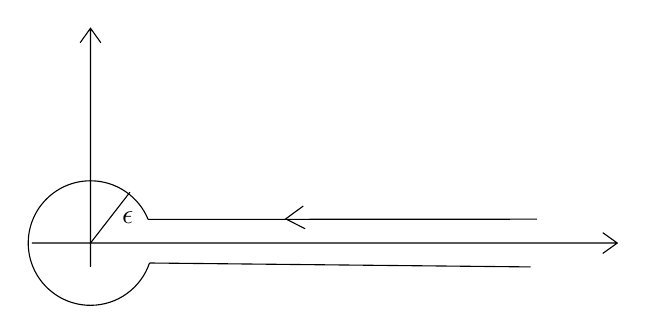
\begin{tikzpicture}[x=0.75pt,y=0.75pt,yscale=-1,xscale=1]
%uncomment if require: \path (0,300); %set diagram left start at 0, and has height of 300

%Shape: Axis 2D [id:dp9785911867399795] 
\draw  (220.8,168.5) -- (502.8,168.5)(249,65) -- (249,180) (495.8,163.5) -- (502.8,168.5) -- (495.8,173.5) (244,72) -- (249,65) -- (254,72)  ;
%Shape: Arc [id:dp1302548314750347] 
\draw  [draw opacity=0] (277.43,178.11) .. controls (273.42,189.96) and (262.21,198.5) .. (249,198.5) .. controls (232.43,198.5) and (219,185.07) .. (219,168.5) .. controls (219,151.93) and (232.43,138.5) .. (249,138.5) .. controls (261.53,138.5) and (272.27,146.18) .. (276.76,157.1) -- (249,168.5) -- cycle ; \draw   (277.43,178.11) .. controls (273.42,189.96) and (262.21,198.5) .. (249,198.5) .. controls (232.43,198.5) and (219,185.07) .. (219,168.5) .. controls (219,151.93) and (232.43,138.5) .. (249,138.5) .. controls (261.53,138.5) and (272.27,146.18) .. (276.76,157.1) ;  
%Straight Lines [id:da7349516742118151] 
\draw    (276.76,157.1) -- (464,157) ;
%Straight Lines [id:da49149077320950185] 
\draw    (277.43,178.11) -- (461,180) ;
\draw   (351.53,150.65) -- (343.02,156.87) -- (352.44,161.61) ;
%Straight Lines [id:da007165525380332216] 
\draw    (249,168.5) -- (268,144) ;

% Text Node
\draw (263,152) node [anchor=north west][inner sep=0.75pt]   [align=left] {$\displaystyle \epsilon $};


\end{tikzpicture}

       \end{center}
        

    \end{enumerate}
\end{theorem} 
\begin{proof}\,

    $ \dps\prod_{p\text{ prime}}\frac{1}{1-p^{-s}}=\frac{1}{\dps \prod_{p\text{ primes}}(1-p^{-s})} $,  $ \Re s>1 $ converges absolutely since  $ \dps\sum_{p\text{ prime}}|p^{-s}|=\sum_{p\text{ prime}}p^{-\Re s} $ converges for  $ \Re s>1 $. Hence,  $ F(s)=\dps\prod_{p\text{ prime}}\frac{1}{1-p^{-s}} $ is analytic and nonzero in  $ \Re s>1 $. It remains to prove that  $ \zeta(s)=F(s) $ for  $ \Re s>1 $.
    \begin{align*}
        \zeta_N(s)&:=\prod_{p \leq N,p\text{ prime}}\frac{1}{1-p^s}\\
        &=\prod_{p \leq N,p\text{ prime}}\sum_{k=0}^\infty p^{-ks}\\
        &=\sum_{\substack{n=p_1^{k_1}p_2^{k_2}\cdots p_m^{k_m}\\p_j \leq N,p_j\text{ prime}}}\frac{1}{n^s},\,\Re s>1
    \end{align*}  
    By the fundamental theorem of arithmetic, 
    \[|\zeta(s)-\zeta_N(s)| \leq \sum_{n \geq N}\frac{1}{|n^s|}\rightarrow 0\text{ as }N\rightarrow \infty\]
    which proves (a), and part of (c):  $ \zeta  $ has no zeros in  $ \Re s>1 $.
    
    Define  $ \dps\theta(t)=\sum_{n=-\infty}^\infty e^{-\pi n^2t} $. We next prove that  $ \theta(t)=\dps\frac{1}{\sqrt{t}}\theta(\frac{1}{t}) $,  $ \forall t>0 $.
    
    $ f(x)=exp(-\pi +x^2) $ whose Fourier transform is 
    \[\hat{f}(k)=\int_{-\infty}^\infty f(x)\exp[-2\pi i kx]\dd x=\frac{1}{\sqrt{t}}\exp[-\frac{\pi k^2}{t}]\]
    The Poisson summation formula implies  \begin{equation}\label{eq1:5.4:theta(t)}
        \theta(t)=\dps\sum_{n=-\infty}^\infty e^{-\pi n^2t}=\sum_{n=-\infty}^\infty \frac{1}{\sqrt{t}}\exp[-\frac{\pi k^2}{t}]=\frac{1}{\sqrt{t}}\theta(\frac{1}{t})
    \end{equation} 
    Note that  $ \theta(t)-1=2\dps\sum_{n=1}^\infty e^{-\pi n^2 t} \leq 2\sum_{n=1}^\infty e^{-\pi nt}=2\frac{e^{-\pi t}}{1-e^{-\pi t}} $,  $ \forall t>0 $.

    \ie  $ \theta(t)=1+O(e^{-\pi t}) $   as  $ t\rightarrow \infty  $.
    
    \eqref{eq1:5.4:theta(t)} implies  $ \dps\theta(t)=\frac{1}{\sqrt{t}}[1+O(e^{-\pi/t})] $ as  $ t\rightarrow 0^+ $ $ \Rightarrow  $  $ \dps\theta(t)=O(\frac{1}{\sqrt{t}}) $  as  $ t\rightarrow 0^+ $.
    
    \begin{equation}
        \Gamma(\frac{s}{2})=\int_0^\infty e^{-t}t^{\frac{s}{2}-1}\dd t,\,\Re s>1
    \end{equation}
    Then replace  $ t  $ with  $ \pi n^2 t $. We obtain that  
    \begin{equation}
        \pi^{-\frac{s}{2}}\Gamma(\frac{s}{2})n^{-s}=\int_0^\infty e^{-\pi n^2t}t^{\frac{s}{2}-1}\dd t,\,\Re s>1
    \end{equation}
    Summing over  $ n $ $ \Rightarrow  $   
    \begin{equation}
        \begin{aligned}
            \zeta^*(s)&=\dps\sum_{n=1}^\infty \int_0^\infty e^{-\pi n^2t}t^{\frac{s}{2}-1}t^{\frac{s}{2}-1}\dd t\\
            & \xlongequal{Fubini} \int_0^\infty \left(\sum_{n=0}^\infty e^{-\pi n^2t}\right)t^{\frac{s}{2}-1}\dd t\\
            &=\int_0^\infty\frac{\theta(t)-1}{2}t^{\frac{s}{2}-1}\dd t,\,\Re s>1
        \end{aligned}
    \end{equation}
    Define  $\dps g(t)=\frac{\theta(t)-1}{2} $. Then  $ g(t)=\dps\frac{\frac{1}{\sqrt{t}}\theta(\frac{1}{t})-1}{2}=\frac{1}{\sqrt{t}}g(\frac{1}{t})+\frac{1}{2\sqrt{t}}-\frac{1}{2} $. Therefore, 
    \begin{equation}
        \begin{aligned}
            \zeta^*(s)&=\int_0^1g(t)t^{\frac{s}{2}-1}\dd t+\int_1^\infty g(t)t^{\frac{s}{2}-1}\dd t\\ 
            &=\int_0^1[\frac{1}{\sqrt{t}}g(\frac{1}{t})+\frac{1}{2\sqrt{t}}-\frac{1}{2}]t^{\frac{s}{2}-1}\dd t+\int_1^\infty g(t)t^{\frac{s}{2}-1}\dd t\\ 
            &=-\frac{1}{s}-\frac{1}{1-s}+\frac{1}{2}\int_1^\infty[\theta(t)-1]\cdot[t^{\frac{-s-1}{2}}+t^{\frac{s}{2}-1}]\dd t,\,\Re s>1
        \end{aligned}
    \end{equation}
    which is analytic if we apply Weierstrass theorem to the final integral. So  $ \zeta  $ can be extended to a meromorphic function on  $ \Cbb $, whose poles are  $ 0,1 $.
    
    \eqref{eq:5.4:symmetrized zeta function} implies  $ \zeta^*(s)=\zeta^*(1-s) $.
    
    This combined with Legendre's duplication formula and  $ \dps\frac{1}{\Gamma(1-\frac{s}{2})\Gamma(\frac{s}{2})}=\frac{\sin (\pi \frac{s}{2})}{\pi} $, we obtain that 
    \begin{equation}\label{eq:5.4:symmetry of zeta function}
        \zeta(s)=2^s\pi^{s-1}\sin(\frac{\pi s}{2})\Gamma(1-s)\zeta(1-s),\, s\in \Gamma\setminus\{0,1\}
    \end{equation} 

    $ \zeta^* $ has simple poles at  $ s=0 $ and  $ s=1 $, with residues  $ -1 $ and  $ 1 $ respectively.
    
    $ \zeta(s)=\dps\frac{\pi^{\frac{s}{2}}\zeta^*(s)}{\Gamma(\frac{s}{2})} $ $ \Rightarrow  $  $ \zeta  $ has a simple pole at  $ s=1 $ with residue  $ \dps\frac{\pi^{\frac{1}{2}}}{\Gamma(\frac{1}{2})}=1 $.  $ s=0 $ is a removable singularity since  $ \Gamma(s)=\dps\frac{1}{s} $ as  $ s\rightarrow 0 $. And  $ \zeta(0)=\dps\frac{1\cdot\frac{-1}{s}}{\frac{1}{\frac{s}{2}}}=-\frac{1}{2} $.   
    
    \eqref{eq:5.4:symmetry of zeta function} implies zeros of  $ \zeta $ for  $ \Re s<0 $ are precisely  $ s=-2k $,  $ k\in \Nbb $.
    
    We have proved (b),(c),(e),(f).

    We next prove (g).
    \begin{align*}
        \int_0^\infty\frac{t^{s-1}}{e^t-1}\dd t&=\int_0^\infty t^{s-1}\sum_{n=1}^\infty e^{-nt}\dd t\\
        &\xlongequal{{Fubini}}\sum_{n=0}^\infty\int_0^\infty t^{s-1}e^{-nt}\dd t\\
        &\overset{u=nt }{=}\sum_{n=1}^\infty\frac{1}{n^s}\int_0^\infty u^{s-1}e^{-u}\dd u\\
        &=\Gamma(s)\zeta(s),\,\Re s>1
    \end{align*}
    For  $ \dps\int_C\frac{(-z)^s}{e^z-1}\cdot\frac{\dd z}{z},\,\Re s>1 $, as  $ \epsilon\downarrow 0 $, the contribution from the  circle of radius  $ \epsilon $ $ \rightarrow 0 $.  Then 
    \begin{align*}
        \int_C\frac{(-z)^s}{e^z-1}\cdot\frac{\dd z}{z}&=\int_{-\infty}^0\frac{\exp[s(\ln t-i\pi)]}{e^t-1}\cdot\frac{dd t}{t}+\int_0^\infty \frac{\exp[s(\ln t+i\pi)]}{e^t-1}\cdot\frac{\dd t}{t}\\
        &=(e^{is\pi}-e^{-is\pi})\int_0^\infty\frac{t^{s-1}}{e^t-1}\dd s\\
        &=2i\sin(s\pi)\Gamma(s)\zeta(s),\,\Re s>1
    \end{align*}  
    \begin{equation}\label{eq:5.4:another expandation of zeta function}
        \begin{aligned}
            \Rightarrow \zeta(s)&=\frac{1}{2i\sin(s\pi)\Gamma(s)}\int_C\frac{(-z)^s}{e^z-1}\cdot\frac{\dd z}{z}\\
            &=\frac{\Gamma(z-s)}{2\pi i}\int_C\frac{(-z)^s}{e^z-1}\cdot\frac{\dd z}{z},\,\Re s>1
        \end{aligned}  
    \end{equation}

    For (d), for  $ \forall n\in \Nbb $,
    \begin{equation}
        \begin{aligned}
            \zeta(-n)&\overset{\eqref{eq:5.4:another expandation of zeta function}}{=}\frac{\Gamma(1+n)}{2\pi i}\int_C\frac{(-z)^{-n}}{e^z-1}\dd z\\
            &=\frac{n!}{2\pi i}\int_C\frac{(-z)^{-n}}{z^2}\sum_{m=0}^\infty\frac{B_m}{m!}z^m\dd z\\
            &=n!(-1)^n\frac{B_{n+1}}{(n+1)!}\\
            &=\frac{(-1)^nB_{n+1}}{n+1}\\
            &=\frac{-B_{n+1}}{n+1}
        \end{aligned}
    \end{equation} 
    since  $ B_{2k+1}=0 $ for  $ k\in \Nbb $. 
    \begin{equation}
        \begin{aligned}
            \eqref{eq:5.4:symmetry of zeta function}\Rightarrow\zeta(2n)&=2^{2n}\pi^{2n-1}\sin(\pi n)\Gamma(1-2n)\zeta(1-2n),\,n\in Nbb\\
            &=\frac{(2\pi)^2n(-1)^n}{2(2n-1)!}\cdot\frac{-B_{2n}}{2n}\\
            &=\frac{(-1)^n(2\pi)^{2n}}{2(2n)!}B_{2n},\,n\in \Nbb
        \end{aligned}
    \end{equation}
\end{proof}

\section{Riemann Mapping Theorem}

\subsection{Normal families}
\subsubsection{The Arzela-Ascoli Theorem}
Let  $ \mathscr{F} $ be a family of functions  $ f  $, defined in a fixed region  $ \Omega\subset \Cbb $, with values in a metric space  $ S $. The distance function in  $ S  $ is denoted by  $ d $.

The functions in a family  $ \mathscr{F} $  are said to be \name{equicontinuous} on a set  $ E\subset \Omega $ if for  $ \forall \epsilon>0 $,  $ \exists \delta>0 $ \st  $ d(f(z),f(z_0))<\epsilon  $,  $ \forall z,z_0\in E $ with  $ |z-z_0|<\delta $ and  $ \forall f\in \mathscr{F} $.

\begin{remark}
    Each  $ f  $ in an equicontinuous family is itself uniformly continuous on  $ E $. 
\end{remark}

A family is said to be \name{normal} (or \name{relatively compact}) in  $ \Omega $ if every sequence  $ \{f_n\} $ of functions  $ f_n\in \mathscr{F} $ contains a subsequence which converges uniformly on every compact subset of  $ \Omega $.

\begin{remark}
    This definition does not require the limit functions of the convergent subsequences to be members of  $ \mathscr{F} $. 
\end{remark}
Let  $ E_k:=\Omega\cap \overline{B(0,k)}\cap \{z\in \Cbb:d(z,\partial \Omega) \geq \dps\frac{1}{k}\} $,  $ k\in \Nbb $.

Then  $ E_k  $ is bounded and closed, and hence compact.

$ \forall  $ compact set  $ E\subset \Omega  $ is bounded and has positive distance from  $ \partial \Omega $ $ \Rightarrow  $  $ E\subset E_k $. So the choice of  $ E_k  $ is representative.

Define  $ \delta(a,b)=\dps\frac{d(a,b)}{1+d(a,b)} $. It is easy to check that  $ \delta  $ is a metric and has the advantage of being bounded.

Define  \begin{equation}\label{eq:6.1.1:definition of delta_k in function space}
    \delta_k(f,g)=\dps\sup_{z\in E_k}\delta(f(z),g(z)) ,\,\rho(f,g)=\dps\sum_{k=1}^\infty\delta_k(f,g)2^{-k} 
\end{equation}

It is easy to check that  $ \rho(f,g) $ is finite and is a distance between  $ f $ and  $ g $ on  $ \Omega $.  

\begin{lemma}\label{thm:6.1.1:Lemma of Arzela-Ascoli Theorem}
     $ f_n\rightrightarrows f$ on every compact subset of  $ \Omega  $ if and only if  $ \rho(f_n,f)\rightarrow 0 $ as  $ n\rightarrow \infty $.    
\end{lemma}
\begin{proof}
    "$ \Leftarrow $":  $ \forall \epsilon>0 $,  $ \exists   N\in\Nbb $ \st  $ \rho(f_n,f)<\epsilon $,  $ \forall n \geq\Nbb $.
    
    \eqref{eq:6.1.1:definition of delta_k in function space} implies  $ \delta_k(f_n,f)<2^k\epsilon $, $ \forall n \geq N $ and  $ \forall  $ fixed  $ k\in \Nbb $. Then  $ f_n\rightrightarrows f $ on  $ E_k $ w.r.t.  $ \delta $-metric, and hence w.r.t. the  $ d $-metric. $ \Rightarrow  $  $ f_n\rightrightarrows f $ on every compact subset  $ E $ of  $ \Omega $ since  $ E \subset E_k $ for some  $ k\in \Nbb $.
    
    "$ \Rightarrow $":  $ E_k  $ is a compact subset of  $ \Omega  $  $ \Rightarrow  $  $ f_n\rightrightarrows f  $ on  $ E_k  $ w.r.t.  $ d $-metric, and hence w.r.t.  $ \delta $-metric $ \Rightarrow  $ $ \delta_k(f_n,f)\rightarrow 0 $ as  $ n\rightarrow \infty $ for  $ \forall $ fixed  $ k\in \Nbb $. Then 
    \begin{equation}
        \lim_{n\to\infty}\sum_{n=1}^\infty\delta_k(f_n,f)2^{-k}\xlongequal{DCT}\sum_{n=1}^\infty\lim_{n\to\infty}\delta_k(f_n,f)2^{-k}=0
    \end{equation}       
    So  $ \rho(f_n,f)\rightarrow 0$ as  $ n\rightarrow \infty $.  
\end{proof}
\begin{theorem}\label{thm:6.1.1:normalness equivalent to precompactness}
    A family  $ \mathscr{F} $ is normal iff its closure  $ \overline{\mathscr{F}} $ w.r.t.  $ \rho $ is compact.   
\end{theorem}
\begin{proof}
    "$ \Leftarrow $":  $ \overline{\mathscr{F}} $ is compact  $ \Leftrightarrow $  $ \forall  $ infinite sequence of  $ \overline{\mathscr{F}} $ has a limit point in  $ \overline{\mathscr{F}} $. So from the lemma \ref{thm:6.1.1:Lemma of Arzela-Ascoli Theorem} $ \overline{\mathscr{F}} $ is normal follows. Then  $ \mathscr{F} $ is normal.
    "$ \Rightarrow $": For  $ f_n\in \overline{\mathscr{F}} $,  WLOG we assume  $ f_n\in \overline{\mathscr{F}}\setminus\mathscr{F} $ for all large  $ n $. Then  $ \forall n\in \Nbb $,  $ \exists \tilde{f}_n\in \mathscr{F} $ \st  $ \rho(f_n,\tilde{f}_n)<\dps\frac{1}{n} $. $ \mathscr{F} $ is normal  $ \Rightarrow  $   $ \{\tilde{f}_n\} $ has a convergent subsequence  $ \{\tilde{f}_{n_k}\}_{k\in\Nbb} $. \ie  $ \tilde{f}_{n_k}\rightrightarrows f\in \overline{\mathscr{F}} $ on every compact  subset of  $ \Omega $. From the lemma \ref{thm:6.1.1:Lemma of Arzela-Ascoli Theorem}  $ \rho(\tilde{f}_{n_k},f)\rightarrow 0 $ as  $ k\rightarrow \infty $ $ \Rightarrow  $ $ \rho(f_{n_k},f)\rightarrow 0 $  as  $ k\rightarrow \infty $ since 
    \begin{equation}
        \rho(f_{n_k},f) \leq \rho(f_{n_k},\tilde{f}_{n_k})+\rho(\tilde{f}_{n_k},f) \leq \frac{1}{n_k}+\rho(\tilde{f}_{n_k},f)
    \end{equation}            
\end{proof}

\begin{theorem}\label{thm:6.1.1:totally bounded is the same w.r.t rho and d}
    The family  $ \mathscr{F} $ is totally  bounded w.r.t.  $ \rho $ iff for  $ \forall  $ compact set  $ E\subset \Omega$ and  $ \forall \epsilon>0 $,  $ \exists f_1,f_2,\cdots,f_n\in \mathscr{F} $ \st every  $ f\in \mathscr{F} $ satisfies  $ d(f,f_j)<\epsilon $ on  $ E $ for some  $ j $.        
\end{theorem}
\begin{proof}
    "$ \Rightarrow $":  $ \mathscr{F} $ is totally bounded $ \Rightarrow  $  $ \forall \epsilon>0 $,  $ \exists f_1,\cdots,f_n\in \mathscr{F} $ \st  $ \forall f\in \mathscr{F} $,  $ \rho(f,f_j)\epsilon $ for some  $ f_j $.  Then \eqref{eq:6.1.1:definition of delta_k in function space} implies  $ \delta_k(f,f_j)<2^k\epsilon $  for each fixed  $ k\in \Nbb $ $ \Rightarrow  $  $ \delta(f(z),f_j(z))<2^k\epsilon $,  $ \forall z\in E_k $ $ \Rightarrow  $  $ d(f(z),f_j(z))<\dps\frac{2^k\epsilon}{1-2^k\epsilon},\,\forall z\in E_k $,  $ \forall k $ fixed and  $ \epsilon  $ small enough.
    
    "$ \Leftarrow $" Fix  $ \epsilon>0 $, pick  $ k_0\in \Nbb $ \st  $ 2^{-k_0}<\dps\frac{\epsilon }{2} $.  $ \forall f\in \mathscr{F} $,  $ \exists j_0\in \{1,2,\cdots,n\} $ \st  $ \delta(f(z),f_{j_0}(z)) \leq d(f(z),f_{j_0}(z))<\dps\frac{\epsilon}{2k_0} $,  $ \forall z\in E_{k_0} $. Then  $ \delta_k(f,f_{j_0})<\dps\frac{\epsilon}{2k_0} $,  $ \forall k \leq k_0 $. $ \Rightarrow  $  $ \rho(f,f_{j_0})<\dps k_0\cdot\frac{\epsilon}{2k_0}+2^{-k_0}<\epsilon $    
\end{proof}

\begin{theorem}[Arzela-Ascoli Theorem]\label{thm:6.1.1:Arzela-Ascoli theorem}
    A family of continuous functions with values in a complete metric space  $ S  $ is normal in the region  $ \Omega\subset\Cbb  $ iff (1)  $ \mathscr{F} $ is equicontinuous on every compact set  $ E\subset \Omega $. (2)  $ \forall z\in \Omega  $,  $ \{f(z):f\in \mathscr{F}\} $ lie in a compact subset of  $ S $.    
\end{theorem}
\begin{proof}
    "$ \Rightarrow $":  $ \mathscr{F} $ is normal  $ \overset{\text{theorem \ref{thm:6.1.1:normalness equivalent to precompactness}}}{\Rightarrow} $ $ \overline{\mathscr{F}} $ is compact w.r.t. $ \rho $  $ \Rightarrow $ $ \overline{\mathscr{F}} $ is totally bounded w.r.t. $ \rho $  $ \Rightarrow $  $ \mathscr{F} $ is totally bounded w.r.t.  $ d $ by theorem \ref{thm:6.1.1:totally bounded is the same w.r.t rho and d}.
    
    Let  $ E\subset \Omega  $ be compact.  $ \forall \epsilon>0 $, determine  $ f_1,\cdots,f_n\in \mathscr{F} $ as in the previous theorem.  $ \mathscr{F}$ is equicontinuous on  $ E $ $ \Rightarrow  $ $ \exists  \delta>0$ \st 
    \[d(f_j(z),f_j(z_0))<\epsilon,\,\forall z,z_0\in E\text{ with }|z-z_0|<\delta\]
     $ \forall f\in \mathscr{F} $. Let  $ f_{j_0} $ be the corresponding  $ f_j  $ from the previous theorem. Then 
     \begin{equation}
        d(f(z),f(z_0)) \leq d(f(z),f_{j_0}(z))+d(f_{j_0}(z),f_{j_0}(z_0))+d(f_{j_0}(z_0),f(z_0))<3\epsilon
     \end{equation}      
    So we prove (1). To prove (2), we prove  $ \overline{\{f(z):f\in \mathscr{F}\}} $ is compact. Let  $ \{\omega_0\} $ be a sequence in  $ \overline{\{f(z):f\text{ in } \mathscr{F}\}} $. Then  $ \forall \omega_n $,  $ \exists  f_n\in \mathscr{F}  $ \st  $ d(f_n,\omega)<\dps\frac{1}{n} $. $ \mathscr{F} $ is normal $ \Rightarrow $ $ \exists  $ convergent subsequence  $ \{f_{n_k}(z)\} $ $ \Rightarrow  $ $ \{\omega_{n_k}\}  $ converges to the same value.  
    
    "$ \Leftarrow $" Choose any sequence  $ \{\zeta_j\} $ which is dense in  $ \Omega $. Let  $ \{f_n\} $ be any sequence in  $ \mathscr{F} $.
    
    $ \{f_n(\zeta_1)\}_{n\in \Nbb} $ is in a compact subset of  $ S $. $ \Rightarrow  $  $ \exists  $ a convergent subsequence  $ \{f_{n,1}(\zeta_1)\}_{n\in \Nbb} $. 

    $ \{f_{n,1}(\zeta_1)\}_{n\in \Nbb} $ is in a compact subset of  $ S $. $ \Rightarrow  $  $ \exists  $ a convergent subsequence  $ \{f_{n,2}(\zeta_1)\}_{n\in \Nbb} $ $ \cdots $ 

    Continue this steps and we obtain  the subsequence  $ \{f_{n,n}\} $ that converges at each  $ \zeta_j $.
    
    Let  $ E\subset \Omega  $ be compact  $ \Rightarrow  $  $ d(E,\partial \Omega)>0 $ $ \Rightarrow  $  $ r:=\dps\frac{d(E,\partial \Omega)}{2} $,  $ K=\dps\bigcup_{z\in E}B(z,r) $ has closure  $ \overline{K}\subset \Omega $.
    
     $ \mathscr{F} $ is equicontinuous on  $ \overline{K} $ $ \Rightarrow $  $ \forall \epsilon>0 $,  $ \exists \delta<r $ \st   
    \begin{equation}\label{eq:6.1.1:1}
        d(f(z),f(z_0))<\frac{\epsilon}{3},\,\forall z,z_0\in \overline{K}\text{ with  $ |z-z_0|<\delta $}
    \end{equation}
     $ \forall z\in E $,  $ B(z,\delta ) $ contains some  $ \zeta_j  $  $ \Rightarrow  $  $ B(\zeta_j,\delta ) $ contains  $ z $.
     
    $ E $ is compact  $ \Rightarrow  $  $ \exists N\in \Nbb  $ \st  $ E\subset \dps\bigcup_{j=1}^N B(\zeta_j,\delta) $ for some  $ \zeta_1,\zeta_2,\cdots,\zeta_N $. By the construction  of  $ f_{n,n} $,  $ \exists N_\epsilon\in \Nbb  $ \st   
    \[\dd(f_{n,n}(\zeta_j),f_{m,m}(\zeta_j))<\frac{\epsilon}{3},\,\forall m,n \geq N_\epsilon,\,\forall j=1,2,\cdots,N\]
     $ \forall z\in E $,  $ \exists \zeta_{j_0}=\zeta_{j_0}(z)$ \st  $ |z-\zeta_{j_0}|<\delta $ for some  $ j_0\in\{1,2,\cdots,N\} $.  
     \[\eqref{eq:6.1.1:1}\Rightarrow \dd(f(z),f(\zeta_{j_0}))<\frac{\epsilon}{3},\,\forall f\in \mathscr{F}\]
    Then
    \begin{equation*}
        \begin{aligned}
            \dd(f_{n,n}(z),f_{m,m}(z)) &\leq \dd (f_{n,n}(z),f_{m,m}(\zeta_{j_0}))+\dd(f_{n,n}(\zeta_{j_0}),f_{m,m}(\zeta_{j_0}))+\dd(f_{m,m}(\zeta_{j_0}),f_{m,m}(z)) \\
            &<\epsilon,\qquad \forall m,n \geq N_\epsilon
        \end{aligned}
    \end{equation*}    

    So  $ \{f_{n,n}\} $ is uniformly Cauchy on  $ E $ $ \Rightarrow  $  $ \{f_{n,n}\} $ converges uniformly on  $ E $.
    \begin{remark}
        In the text, p.233, it is erroneously assumed that  $ \zeta_k\in E $. 
    \end{remark}    
\end{proof}